\documentclass[tikz,border=3pt]{standalone}
\usepackage{tikz}
\usetikzlibrary{arrows.meta,positioning,shapes.geometric}
\begin{document}
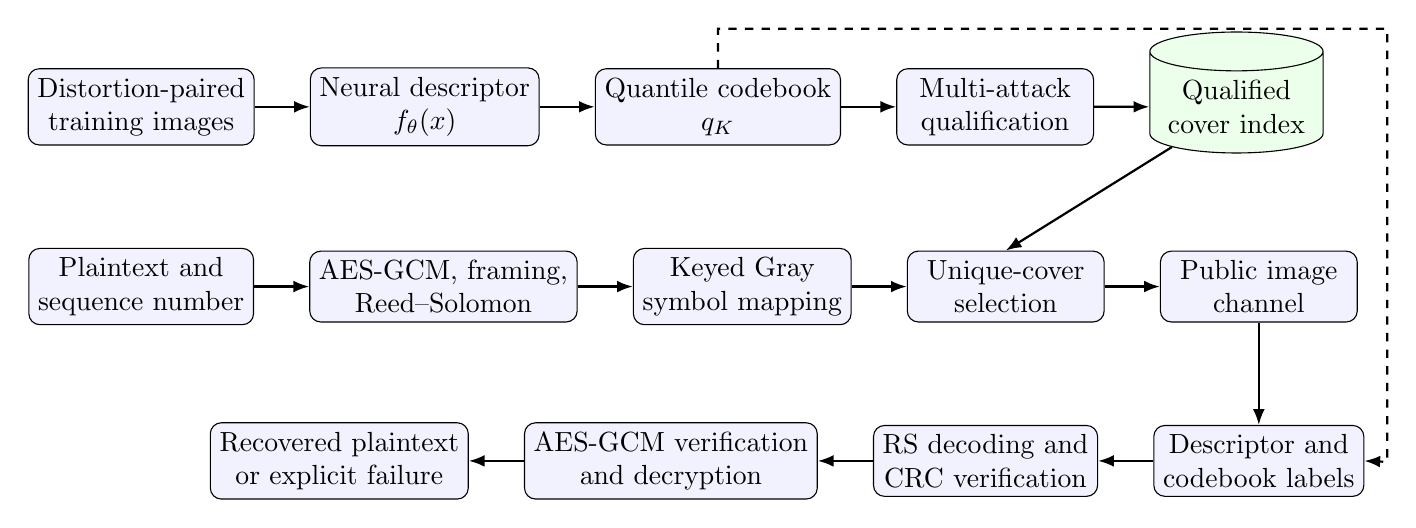
\begin{tikzpicture}[
  node distance=5mm and 7mm,
  box/.style={draw, rounded corners, align=center, minimum height=9mm,
    minimum width=25mm, fill=blue!5},
  store/.style={draw, cylinder, shape border rotate=90, aspect=0.25,
    align=center, minimum height=11mm, minimum width=22mm, fill=green!8},
  arrow/.style={-{Latex[length=2mm]}, thick},
  dashedarrow/.style={-{Latex[length=2mm]}, thick, dashed}
]
\node[box] (train) {Distortion-paired\\training images};
\node[box, right=of train] (encoder) {Neural descriptor\\$f_\theta(x)$};
\node[box, right=of encoder] (quantile) {Quantile codebook\\$q_K$};
\node[box, right=of quantile] (qualify) {Multi-attack\\qualification};
\node[store, right=of qualify] (index) {Qualified\\cover index};

\node[box, below=13mm of train] (payload) {Plaintext and\\sequence number};
\node[box, right=of payload] (aead) {AES-GCM, framing,\\Reed--Solomon};
\node[box, right=of aead] (mapping) {Keyed Gray\\symbol mapping};
\node[box, right=of mapping] (select) {Unique-cover\\selection};
\node[box, right=of select] (channel) {Public image\\channel};

\node[box, below=13mm of channel] (classify) {Descriptor and\\codebook labels};
\node[box, left=of classify] (decode) {RS decoding and\\CRC verification};
\node[box, left=of decode] (decrypt) {AES-GCM verification\\and decryption};
\node[box, left=of decrypt] (output) {Recovered plaintext\\or explicit failure};

\draw[arrow] (train) -- (encoder);
\draw[arrow] (encoder) -- (quantile);
\draw[arrow] (quantile) -- (qualify);
\draw[arrow] (qualify) -- (index);
\draw[arrow] (payload) -- (aead);
\draw[arrow] (aead) -- (mapping);
\draw[arrow] (mapping) -- (select);
\draw[arrow] (index) -- (select.north);
\draw[arrow] (select) -- (channel);
\draw[arrow] (channel) -- (classify);
\draw[arrow] (classify) -- (decode);
\draw[arrow] (decode) -- (decrypt);
\draw[arrow] (decrypt) -- (output);
%\draw[dashedarrow] (quantile) -- (classify.north);
\draw[dashedarrow] (quantile.north) -- ++(0,0.5cm) -- ++(8.5cm,0) -- ++(0,-5.5cm) -- (classify.east);
\end{tikzpicture}
\end{document}
